\documentclass[11pt]{article}
\usepackage{graphicx}
\usepackage{listings}
\usepackage{color}
\usepackage[margin=1.2in]{geometry}
\usepackage{courier}
\usepackage{float}
\usepackage[toc,page]{appendix}
\usepackage{amsmath}
\usepackage{hyperref}
\usepackage{booktabs}
\usepackage{multirow}
\usepackage{setspace}
\usepackage{enumitem}

\definecolor{codegreen}{rgb}{0,0.6,0}
\definecolor{codeblack}{rgb}{0,0,0}
\definecolor{codered}{rgb}{0.867,0,0}
\definecolor{backcolour}{rgb}{ 0.95,0.95,0.95}
\definecolor{codeorange}{rgb}{1,0.447059,0}
\definecolor{codegrey}{rgb}{0.1, 0.1, 0.1}
\definecolor{codeblue}{rgb}{0.29, 0.52, 0.56}
\lstdefinestyle{mystyle}{
    basicstyle=\ttfamily\color{codeblack},
    backgroundcolor=\color{backcolour},   
    commentstyle=\color{codered},
    keywordstyle=\color{codeorange},
    numberstyle=\color{codeblack},
    stringstyle=\color{codegreen},
    breakatwhitespace=false,         
    breaklines=true,                 
    captionpos=b,                    
    keepspaces=true,                 
    numbers=left,                    
    numbersep=10pt,                  
    showspaces=false,                
    showstringspaces=false,
    showtabs=false,                  
    tabsize=3
}
 
\lstset{style=mystyle}


\twocolumn
\begin{document}
\title{CCE3015 - Programming Parallel Architectures - Assignment Part 2 - Report - The Parallel Implementation}
\author{Daniel Cauchi}
\date{}
\maketitle

\section{Introduction} \label{intro}
This report is a continuation of the first Assignment of this unit. For a more detailed introduction to the problem, this can be found in part 1. In this second part we implement the same binary tree fractal but using CUDA, such that we run it in parallel on the GPU, rather than serially on CPU. Benchmarks on GPU and CPU were made on a \textit{GeForce GTX TITAN Black} and an \textit{Intel (R) Core (TM) i5 CPU 760 2.8GHz} respectively. An image of an example target tree is  found in Figure \ref{general explanation}. This report will first discuss the implementation and optimizations made alongside difficulties inherent with the problem itself, followed by a comparison of results between the parallel and serial implementation.Any graphs shown will be made using using Matplotlib \cite{matplotlib}.

\begin{figure}
	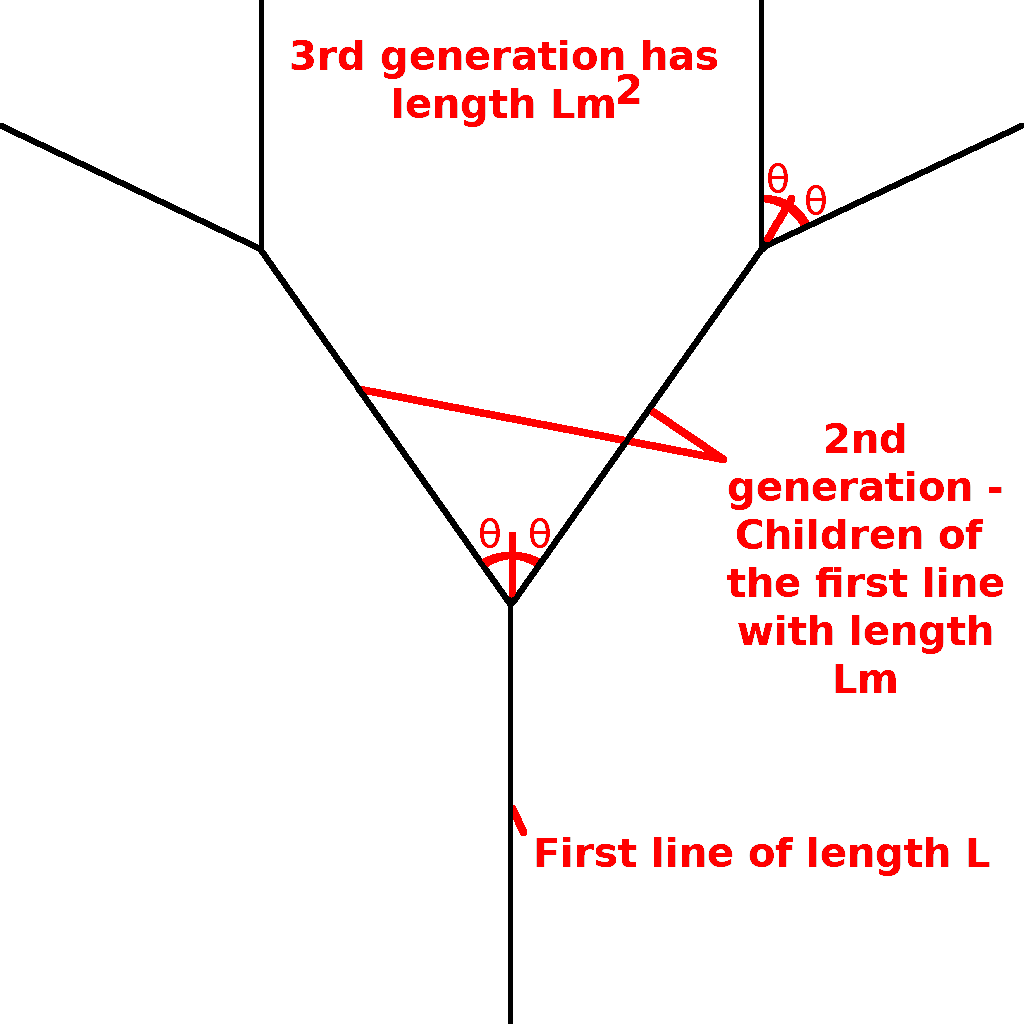
\includegraphics[width=.95\linewidth]{Images/GeneralExplanation.png}
	\centering
	\caption{A fractal generated by the program, with $\theta=30$, $m=0.6$ and $n=3$}
	\label{general explanation}
\end{figure}

\section{Implementation}
As in the first part, we separate this problem into 2 parts, and then further separated into a pipeline. We do a similar separation in this section. In the first part we generate the points, and in the second part we render them. The pipelines for the 2 parts however will however slightly differ. With regards to the inputs, these are the same as the serial implementation (note that we do not have an initial length as this is inconsequential, due to us stretching the image to fit the image):

\begin{itemize}
	\item Output Image Width W
	\item Output Image Height H
	\item Length multiplier per iteration \textit{m}
	\item Rotation per iteration (in degrees) $\theta$
	\item Number of iterations n
\end{itemize}

The following is the pipeline for the first part of the problem. We put a maximum kernel threads at 512, the reason for this is to make it compatible with older hardware.

\begin{enumerate}
	\item Allocate memory in the device for the cosine and sine maps, which map an angle in degrees to an angle in radians. Thus these are of type \textit{float}. We make these of size 512 each so as to avoid warp divergence later on. Thus we have to allocate $4\ bytes * 512 * 2 = 4KB$ for these, which is very small, and thus can fit in shared memory.
	
	\item Allocate memory in GPU for the list of angles and coordinates. Each of these arrays is of size $2^n$, where n is the number of iterations. However, while the list of angles is of type \textit{short} (since these are in degrees, and are used as the indexes to the cosine and sine maps), the list of coordinates are of type \textit{float}. The list of coordinates needs to be multiplied by 2, as we have one for the X-coordinate and one for the Y-coordinate. Thus, with regards to the angles list, we need to allocate $2*2^n\ bytes$ and for each coordinate we allocate $2*4*2^n\ bytes$, totalling to $10*2^n\ bytes$. At 26 iterations, this totals to \textit{640 MB}.
	
	\item Initialize first 2 indexes of the angles and coordinates with both degrees being 0, and the first 2 coordinates being $(0,0)$ and $(0,1)$, representing a straight line straight trough the middle of the image. This is done by simply making an array of size 2 for each of the three lists in the host, then copying them over to the device.
	
	\item Populate the sine and cosine maps, by calling a kernel with 512 threads, where each thread initializes a single index of each map. 512 is a good thread number since it is a multiple of 32 (warp size).
	
	\item The next step is to calculate the coordinates. This is divided into two steps for optimisation. The first step is to calculate the first 2048 coordinates. This is done in a single kernel call, with 512 threads. At each step, we compute as much as was computed at the previous step * 2. This is because index i depends on $\lfloor i\%2 \rfloor$. Thus we need to compute the coordinates iteration by iteration, doing a \textit{syncthreads} call after each one, which is an unfortunate limitation to our problem. Each thread computes 2 coordinates. We say that we calculate the first 2048 points because 512 threads can compute up to 1024 coordinate at the same time, however the first 1024 coordinates are computed by the first few iterations, with 512 coordinates being computed by the iteration before the last. As an optimization, whose performance improvement will be discussed in the next section, we put the sine and cosine maps in shared memory. This is the reason we used a list of size 512 for these, so that we can avoid an if statement, and each thread can perform one calculation without running into problems.
	
	After these first 2048 coordinates, we must synchronize the iterations by issuing separate kernel calls. Thus, each call has as many threads as there are coordinates to compute (divided by 2 since each thread computes 2 points). We keep the number of threads per kernel at 512, and multiply the number of kernels by 2 for each iteration.
	
	\item Since we will not need them any more, we can free the memory allocated for the sine map, the cosine map and the angles list.
	
	
	
	\item Next, we must find the boundaries of the coordinates, so that we can then determine where each coordinate should be on the image. This is done by finding the minimum and maximum Y coordinate, and the maximum X coordinate. Since $max(X)=-min(X)$, we only look once for the maximum X and take the negative of this to get the minimum. Thus, for this process, we need to allocate an array of 3 floats for the results, and a \textit{working} array of floats which needs to be half of $2^n$ which is $2^{n-1}$.
	
	\item The \textit{max} and \textit{min} functions are very similar hence we will discuss one of them, as the other can be inferred very easily from the first. The structure of the process is also similar to generating the points, but opposite. By this we mean that while when generating the points we start from a small array then expand by double each time to fill the entire array, here we start with the big array first and then half it each time until we are left with one value. We do not actually half it of course, but rather we only use half of what we used in the previous iteration. As the iterations depend on each other, we once again run into the problem that we need to synchronize. When we have an array bigger than 1024, we must synchronize by doing individual kernel calls per iteration. As for the last 1024, we can do these in a single kernel and synchronize with \textit{syncthreads}.
	
	In order to avoid if statements, and thus avoid warp divergence we use the following method to get the maximum of 2 values:\\
	$list[index] = list[ index*2 + (list[index*2] < list[index*2 + 1]) ]$
	
	Here is what is happening, with an example. Lets say that we have a list where: list[10] = 58, list[11] = 100, and we need to compare indexes 10 and 11. The result of these will go to list[5], hence it would be performed by thread 5. Thus, we have:\\
	$list[5] = list[5*2+(58<60)]$\\
	Since 60 is greater than 58, the expression $58<60$ will return 1, and thus we end up with $list[5] = list[11]$, which is what is desired. Meanwhile, we would have ended up with $list[5] = list[10]$ if $list[10]$ was greater than (or equal to) $list[11]$. Consequently, we avoid if statements and thus warp divergence.
	
	\item After finding the minimum and maximum, we can now copy these over to the host to perform 4 calculations which we will need to convert the coordinates from coordinate space to image pixel space. At this point, we can also free the arrays we used for finding the minimum and maximum values.
	
	\item The final function we need to do is to convert the coordinates to image space. To do this we launch as many threads as we have points and each thread does a simple multiplication and addition to map to pixel space.
\end{enumerate}

A note on the methods above, specifically for generating the points and finding the minimum and maximum: sometimes we do not need to launch the kernels which do iteration by iteration. These are in cases where we do not have many points to generate and a single kernel with 512 threads would suffice.

The next part is to synthesize the image. The following are the steps taken:

\begin{enumerate}
	\item Allocate an array of short in the device memory of size $W*H$. These represent our pixels. The value of these pixels will be 0 or 255, 0 meaning black and 255 meaning white.
	
	\item Next we initialize all the pixels to 255, by issuing as many as many threads as there are pixels, floored to the next multiple of 512, so each thread initializes a single pixel.
	
	\item The next step is the synthesis function. This is the most complex of all and we will see it is also the one which takes the most time. Firstly, we initialize this with as many threads as there are lines, since each line needs to be drawn on the image. Before we explain the algorithm itself, lets reiterate how we draw a line between 2 points. Quoting directly from part 1 of this assignment: "[S]ay we have only the first line to draw, and we move in the x-axis. If this is done, then we end up with just 1 pixel drawn. Therefore, the approach taken is to move pixel by pixel in the axis for which the distance between the points in that axis is biggest. So for a mostly horizontal line, we move in the x-axis, and if we have a mostly vertical line, we move pixel by pixel in the y-axis." To determine how much is needed to be moved in the other axis, this is calculated by doing the distance between the points in that axis divided by the distance between the points in the bigger axis.
	
	Thus, we first find the absolute difference between the points in both the x and y axis, using the following absolute function which avoids if else statements:
	
	$diffX = (x1-x2)*(x1\ge x2) +\\ (x2-x1)*(x2>x1)$
	
	With this obtained for both the x and y axis, we find how much we need to increase (or decrease) from the first point to the second point in both axes, using a similar method without using if statements. Finally, we can draw the image. Here unfortunately we will have to use a for loop, to go from the first point to the last.
	
	\item Lastly we can copy the image array over to the host and clean up the remaining device memory used.
\end{enumerate}
\section{Theoretic Speed-up}
In this section we see what the theoretic speed-up should be of the parallel implementation. We do this for part 1 of our problem, as part 2 is difficult to predict due to a loop where the number of operations is difficult to determine. We further split part 1 into its different functions to see how long each should take. This is done by checking how many operations need to be computed by the Titan Black, which uses compute capability 3.5 and has 15 multiprocessors.

\subsection{\textit{populate\_sin\_cos\_maps}}
Here, each thread computes a sine and a cosine function and we have 512 threads. This means that this function should take:

\[\frac{N/A}{M} = \frac{512 * 2 / 32} {15} = 2.133 \quad ClockCycles\]

Where 
\begin{itemize}
	\item N = Number of times operation O needs to execute
	\item A = Amount of times operation O can be performed per clock cycle per multi-processor
	\item M = Number of multi-processors
\end{itemize}

\subsection{\textit{calculate\_points}}
Here we have to perform 3 bit shifts (if we consider multiplication of an integer by 2 also as a bit shift), 2 integer addition, 5 float additions and 4 floating point multiplication for every 2 points.

\[ \frac{((3/644) + (2/160) + (5/192) + (4/192))2^{n-1}}{15} \]
\[=4.26889*10^{-3}*2^{n-1} \quad ClockCycles\]

\subsection{\textit{calculateMin} and \textit{calculateMax}}
These 2 functions have the same operations and are executed 3 times in total for as many times as we have points. Here we have 3 integer additions and 1 multiplication, 3 bit shifts and 1 comparison, hence we get:

\[3\frac{3/160 + 1/32 + 3/644 + 1/160}{15}2^{n}\]
\[=3*0.00406056*2^n \quad ClockCycles\]

\subsection{\textit{map\_points\_to\_pixels}}
This last function has 2 float multiplications and 2 float additions per points, meaning:
\[\frac{2/192 + 2/192}{15}2^{n}\]
\[=\frac{1}{720}2^n \quad ClockCycles\]
\section{Testing and Results} \label{results}


\section{Conclusion}
This concludes this report for the parallel implementation of creating tree fractals. A description of how this solution can be implemented in parallel on GPU using CUDA was discussed. Difficulties and Shortcomings of the algorithm were discussed and a comparison to the serial implementation was shown so as to show the obtained speed-up and scalability.

\bibliography{main}
\bibliographystyle{ieeetr}

\onecolumn
\section*{Appendix}
\appendix
\section{Profiler output}
\begin{figure}[H]
	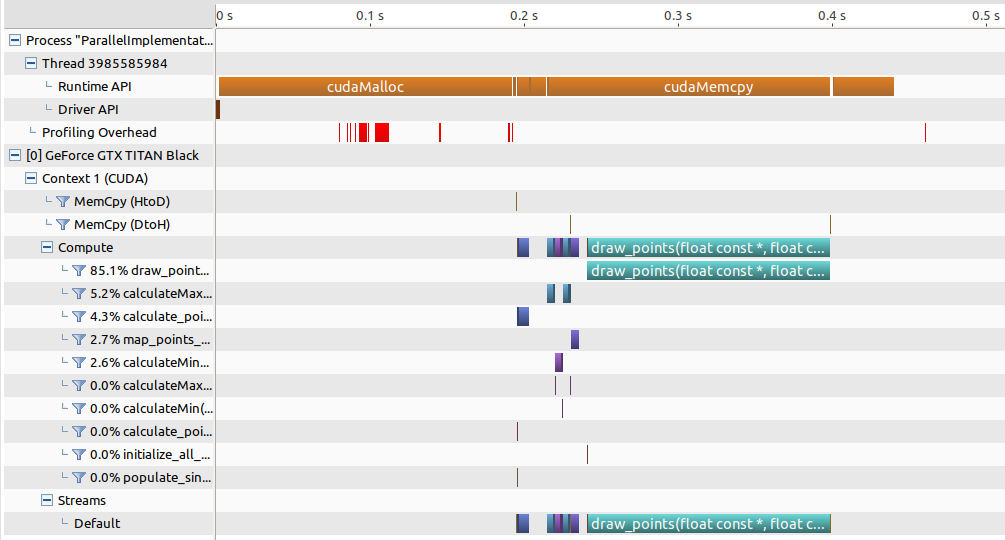
\includegraphics[width=.95\linewidth]{Images/500x500_1_90_26_profilerOutput.png}
	\centering
	\caption{Profiler timeline output for parameters WxH=500x500 m=1 $\theta$=90 n=26 both with sin and cosine in shared memory and without in the \textit{compute\_points} function (no difference was found)}
	\label{fig:profiler}
\end{figure}

\pagebreak

%\input{Subfiles/Appendix}

\end{document}